\documentclass[aspectratio=169]{beamer}
\mode<presentation>
%\usetheme{Warsaw}
%\usetheme{Goettingen}
\usetheme{Hannover}
%\useoutertheme{default}

%\useoutertheme{infolines}
\useoutertheme{sidebar}
\usecolortheme{dolphin}


\setbeamersize{sidebar width left=0pt} % to remove the sidebar
\beamertemplatenavigationsymbolsempty % To remove the navigation symbols on the bottom right.
\setbeamersize{text margin left=10mm,text margin right=10mm} % Specify margins

\usepackage{amsmath}
\usepackage{amssymb}
\usepackage{listings}
\usepackage{enumerate}
\usepackage{hyperref}
\hypersetup{
    colorlinks=true,
    linkcolor=blue,
    filecolor=magenta,      
    urlcolor=cyan,
}


\usepackage{tabularray}
%\SetTblrInner{row{1}={blue9}}
\usepackage{booktabs}% http://ctan.org/pkg/booktabs
\newcommand{\tabitem}{~~\llap{\textbullet}~~}
 
\urlstyle{same}

%some bold math symbosl
\newcommand{\Cov}{\mathrm{Cov}}
\newcommand{\Var}{\mathrm{Var}}
\newcommand{\brho}{\boldsymbol{\rho}}
\newcommand{\bSigma}{\boldsymbol{\Sigma}}
\newcommand{\btheta}{\boldsymbol{\theta}}
\newcommand{\bbeta}{\boldsymbol{\beta}}
\newcommand{\bmu}{\boldsymbol{\mu}}
\newcommand{\bW}{\mathbf{W}}
\newcommand{\one}{\mathbf{1}}
\newcommand{\bH}{\mathbf{H}}
\newcommand{\by}{\mathbf{y}}
\newcommand{\bolde}{\mathbf{e}}
\newcommand{\bx}{\mathbf{x}}

\newcommand{\cpp}[1]{\texttt{#1}}

%--------------------------------------------------
\providecommand{\abs}[1]{\lvert#1\rvert}
\providecommand{\norm}[1]{\lVert#1\rVert}
\providecommand{\Blue}[1]{\textcolor{blue}{#1}}
\providecommand{\Red}[1]{\textcolor{red}{#1}}
\newcommand{\celsius}{\ensuremath{^\circ}C}
\newcommand\thfore{\mathord{\therefore}\,}
%--------------------------------------------

\title{Lecture 16. Logical Arguments}

%\author{BongSik Kim}

%%%%%%Ref: Levin p204---

\date{``My theory says: if P, then Q. 
I design an experiment to see if Q obtains. 
It does. Therefore, P is true."\\
\medskip

\Blue{Is  this argument valid?}}
 %Sadly, this conclusion is logically incorrect. 
 %Q might hold for a variety of reasons having little or nothing to do with my theory. 
 %Yet scientists make this mistake all the time, which led philosopher Karl Popper 
 %to argue that the method of science is—or at least should be—falsification. Popper insisted 
 %that one can never prove that a theory is true, because that would require you to test it 
 %in every conceivable circumstance, which is impossible. But just a single counterexample can 
 %prove a theory false.
 %https://www.scientificamerican.com/article/the-false-logic-behind-science-denial/

%\logo{\includegraphics[height=0.5cm]{Logo_PPT.pdf}}

\begin{document}
\frame[plain]{\titlepage}

\begin{frame}[plain]{What is a logical argument?}


\Blue{Logical argument}. A sequence of statements aimed at demonstrating 
    the truth of an assertion
    
 \begin{itemize}
   \item \Blue{Premise} (or, assumption, hypothesis):
    A statement in an argument that provides reason or 
    support for the conclusion. There can be one or many premises 
    in a single argument.


   \item \Blue{Conclusion}: A statement in an argument that indicates 
    of what the arguer is trying to convince the reader/listener.
    There can be only one conclusion in a single argument.
  \end{itemize}
  
%\Blue{Formal logic}. The framework for determining the validity or
%invalidity of arguments
%\medskip

\Blue{Proof/Derivation/Logical deduction}. A valid sequence of statements 
used for establishing new mathematical truths (or conclusions or propositions or theorems) 
from acceptable/established mathematical truths (premises or axioms or assumptions)

\end{frame}

\begin{frame}[plain]{}

 \begin{center}
  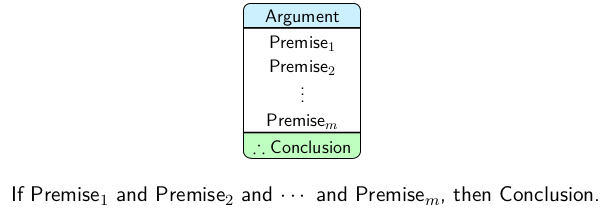
\includegraphics[height=3.5cm]{./img/lecture16-fig1.png}
 \end{center}
 
 For example,
 \medskip
 
 \ \ \ \ \  Every employee who received a large bonus works hard.\\
\ \ \ \ \  Aisha is an employee at the company.\\
\ \ \ \ \ Aisha received a large bonus.\\
\ \ \ \  -------------------------------------------------------------------\\
\ \ \ \ \    $\thfore$ Some employee works hard. 
 
\end{frame}

\begin{frame}[plain]{  }

 %https://www.uky.edu/~rosdatte/phi120/lesson1a.htm#:~:text=A%20premise%20is%20a%20statement,to%20convince%20the%20reader%2Flistener.

 {\bf Example 16.1}.
   Rewrite the following arguments listing the {\bf premise(s)} first 
  and the {\bf conclusion} last.
  Each line should be a single statement written as a complete sentence.
   Feel free to modify the sentences as you deem necessary, without changing their basic meaning
   (not writing a new argument!) 
   Label the premise(s) as $P_1, P_2,$ etc. and the conclusion $C$.
   Leave out any indicator words and any fluff 
   (i.e., sentences which are neither the conclusion nor a premise).
  \medskip
  
  ``Cats with long hair shed all over the house so you should not get a long-haired cat.\\
  I have heard that they also have lots of fleas."\\
  \medskip
  \pause
  
  \begin{itemize}
   \item $P_1$: Long-haired cats shed all over the house.
   \item $P_2$: Long-haired cats have a lot of fleas.
   \item $C$: You should not get a long haired cat.
  \end{itemize}
     
   
\end{frame}

%\begin{frame}[plain]{}

 %\begin{enumerate}
 %  \item Since the housing market is depressed and interest rates are low, 
 %   it's a good time to buy a home.
 %  \item Scientific discoveries are constantly debunking superstitious myths.
 %     Further, science provides the only hope for solving the many problems faced by humankind.
  % Hence, science offers a more accurate view of human life than  any other.
 %\end{enumerate}
% \medskip
 
 %{\bf Assignment.}  Write out two arguments you have encountered in your daily life. 
%  First, write them as you encountered them. Then rewrite them in the format you practiced 
 % in the introductory activity above. 
 % Make sure they are arguments with premises and conclusions.
  
%\end{frame}

\begin{frame}[plain]{Validity of an Argument}

 An argument is \Blue{valid} if the conclusion must be true whenever the premises are all true..
   \begin{itemize}
      \item That is, a valid argument means that no matter what particular
statements are substituted for the statement variables in its
premises, if the resulting premises are all true, then the conclusion is also true
   \end{itemize}
 
{\bf Example 16.2.} Valid or invalid? 
  \begin{itemize}
    \item[(a)] If it is raining, then it is cloudy.\\
              It is raining.\\
              Therefore, it is cloudy. %valid
    \item[(b)] If it is raining, then it is cloudy.\\
              It is not raining.\\
              Therefore, it is not cloudy. %invalid    
    \item[(c)] If $x>2$, then $x^2>4$.\\
              $x\leq 2$.\\
              Therefore,  $x^2\leq 4$. %invalid
  \end{itemize}
   
 \end{frame}
 
\begin{frame}[plain]{How to determine if an argument is valid/invalid?}
 
 {\small 
 \begin{table}
  \centering
  \begin{tabular}{lll}
    \toprule
    \multicolumn{3}{l}{\Blue{Method 1}: Construct a truth table} \\[.5\normalbaselineskip]
    \midrule
    1.~Identify the premises and conclusion. \\[.5\normalbaselineskip]
    2.~Construct a \Red{truth table} for premises and conclusion. \\[.5\normalbaselineskip]
    3.~A row of the truth table in which all the premises are true is
     called a \Red{critical row}. \\
    \tabitem If there is a critical row in which the conclusion is false, 
        then
         the argument is \Red{invalid}. & &\\
    \tabitem If the conclusion in \Red{every} critical row
       is true, then the argument is \Red{valid} & & \\[.5\normalbaselineskip]
    \bottomrule
    \toprule
    \multicolumn{3}{l}{\Blue{Method 2}: Find a counterexample} \\[.5\normalbaselineskip]
    \midrule
    1.~If there is a \Red{counterexample} that has all premises true and false
conclusion, \\
    \ \ \ \ then the argument is \Red{invalid}. \\[.5\normalbaselineskip]
    2.~Failing to find a counterexample does \Red{not} prove that the argument is \Red{valid}.  
      & & \\ [.5\normalbaselineskip] 
    \bottomrule
    \toprule
    \multicolumn{3}{l}{\Blue{Method 3}: Apply the rules of inference} \\[.5\normalbaselineskip]
    \bottomrule
  \end{tabular}

\end{table}
}

\end{frame}


\begin{frame}[plain]{}

 {\bf Example 16.3}. Use a truth table to determine the validity of the argument:\\
   \medskip
   
    \begin{columns}[t] % contents are top vertically aligned
        \begin{column}[c]{2.5cm}
          \ \ \ \ \  $p \rightarrow q\vee \neg r$\\
         \ \ \ \ \  $q \rightarrow p\wedge r$\\
         \ \ \ \  --------------\\
         \ \ \ \ \    $\thfore$ $p\rightarrow r$  
         
        \end{column}\pause 
       \begin{column}[c]{8cm} % each column can also be its own environment  
       
        \begin{center}
          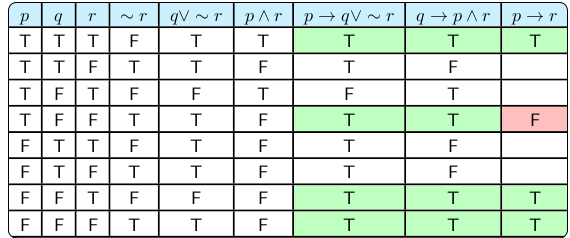
\includegraphics[height=3.5cm]{./img/lecture16-fig2.png}
        \end{center}
             \ \ \   \Red{4th row} (a critical row) has false conclusion. Invalid argument.
        \end{column}
  \end{columns}  
 
\end{frame}

\begin{frame}[plain]{}

%%%%%%%%%%%%%%%%%
\iffalse

{\bf Practice 16.4}.
   Consider the following argument:\\
  \smallskip
  
   \ \ \ ``If you have a current password, then you can log onto the network."\\
   \ \ \ ``You have a current password."\\
   \ \ \  Therefore,\\
   \ \ \  ``You can log onto the network."\\ 
   \medskip
 Write the argument in a logical form and   
  use a truth table to determine the validity of the argument.
 \fi
%%%%%%%%%%%%%%

{\bf Practice 16.4}.
   Consider the following argument:\\
  \smallskip
  
   \ \ \ ``Graphs with high vertex degrees often have high edge weights."\\
   \ \ \ ``Graphs with high edge weights are computationally expensive to traverse."\\
   \ \ \  Therefore,\\
   \ \ \  ``Graphs with high vertex degrees are computationally expensive to traverse."\\ 
   \medskip
 Write the argument in a logical form and   
  use a truth table to determine the validity of the argument.\pause
  \medskip
  
  \begin{itemize}
    \item Premise 1: $X\rightarrow W$
   (``If a graph has high vertex degrees, then it often has high edge weights.")
   \item Premise 2: $W\rightarrow Y$
  (``If a graph has high edge weights, then it is computationally expensive to traverse.")
   \item Conclusion: $X\rightarrow Y$
   (``If a graph has high vertex degrees, then it is computationally expensive to traverse.")
  \end{itemize}
  
  
 \end{frame}
 
 \begin{frame}[plain]{}
 
  \begin{center}
       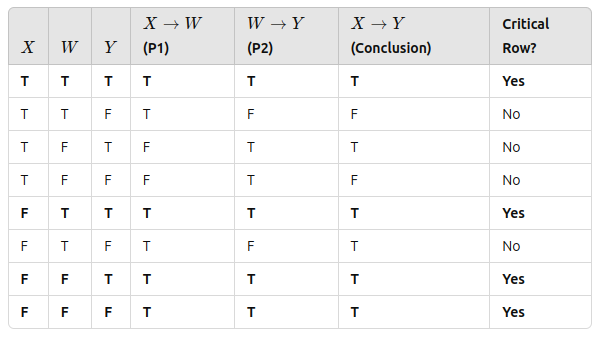
\includegraphics[height=6cm]{./img/lecture16-fig3.png}
     \end{center}
     
   This shows that whenever the premises are true, the conclusion is true, 
   confirming the validity of the argument.
 
\end{frame}


 \begin{frame}[plain]{}
 %SOurce: https://calcworkshop.com/logic/rules-inference/
  
  A \Blue{rule of inference} is a valid argument form that can be used
   to establish logical deductions
   
   \begin{center}
       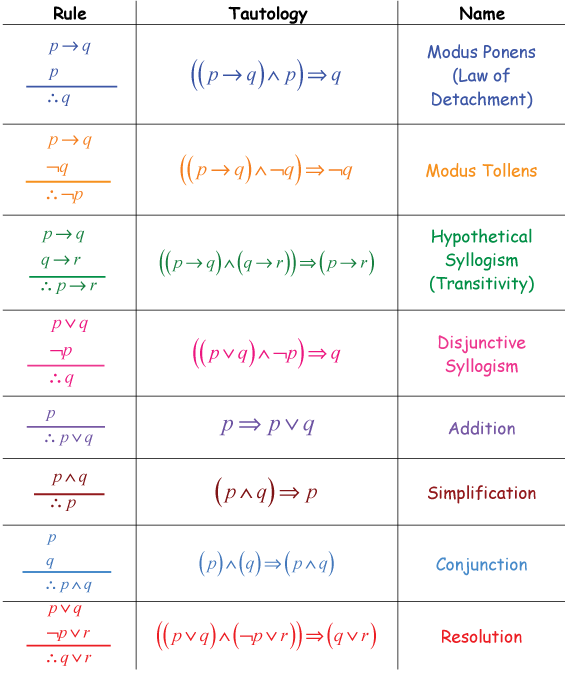
\includegraphics[height=8cm]{./img/lecture16-fig4.png}
     \end{center}
   
 \end{frame}

\begin{frame}[plain]{ }
  
  \begin{itemize}
   \item Note that all rules of inference are tautology.
   \item {\bf Notation:} When a tautology is of the form \Blue{$(C\wedge D)\Rightarrow E$}, we prefer to write as
       \Blue{
       \[ \left. \begin{array}{c}
            C \\ D
           \end{array} \right\}  \Rightarrow E
       \]
       }
      This notation highlights the fact that \Blue{if you know both $C$ and $D$, then 
      you can conclude $E$}.


  \end{itemize}
 
   \vspace{1in}
   
\end{frame}

\begin{frame}[plain]{Modus Ponens}
  
 \Blue{Modus ponens}.
      \[ \Blue{ \left. \begin{array}{c}
             p\rightarrow q \\ p 
           \end{array} \right\}  \Rightarrow q
           }
       \]
      \medskip
      
 % \item {\bf Example} Justify the conclusion: ``If Monique is 18 years old, then she may vote.
 %     Monique is 18 years old. Therefore, monique may vote''.
 
   {\bf Example 16.5.} Justify the conclusion (i.e., determine whether the given argument is valid): 
 %  ``You need a current password to access department machines.
 %   You have a current password. Therefore, You can access department machines.'' 
 ``If the self-drive car detects an obstacle in its path, 
 it will apply the brakes. The self-drive car has detected an obstacle 
 in its path. Therefore, the self-drive car will apply the brakes."
    \pause 
    \medskip
    
     \begin{center}
       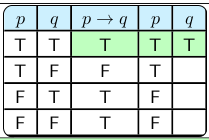
\includegraphics[height=2.7cm]{./img/lecture16-fig5.png}
     \end{center}
  

\end{frame}

\begin{frame}[plain]{Modus Tollens}
  
  \Blue{Modus tollens} (= denial mode). 
    
      \[ \Blue{ \left. \begin{array}{c}
            p\rightarrow q \\  \neg q 
           \end{array} \right\}  \Rightarrow \neg p
           }
       \]
       \medskip
       \pause
       
 {\bf Example 16.6}. Justify the conclusion:
%   ``Our professor does not own a spaceship. If our
%      professor is from Mars, then our professor owns a spaceship. Therefore, our professor
 %     is not from Mars''.
 ``If the self-drive car detects an obstacle in its path, 
 it will apply the brakes.
  The self-drive car has not applied the brakes.
  Therefore, the self-drive car has not detected an obstacle in its path."
  \pause 
    \medskip
    
     \begin{center}
       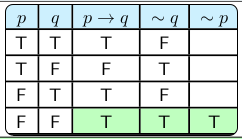
\includegraphics[height=2.7cm]{./img/lecture16-fig6.png}
     \end{center}
  
\end{frame}


 \begin{frame}[plain]{Proof Sequences}
 
 We now have enough tools to derive some new tautologies from old ones. 
 A \Blue{proof sequence} is a sequence of statements with reasons~\footnote{
   logical equivalences
 and inference rules}
 to justify an assertion of the form
 \[ \Blue{[A_1\wedge A_2\wedge \cdots A_n]  \Rightarrow C} \]  
 \pause 
 
{\bf Example 16.7.} Write a proof of sequence for the assertion 
     \[ \left. \begin{array}{c}
            p\vee q \\ \neg p
           \end{array} \right\}  \Rightarrow q
       \]
%Essentiala, sec 1.2 p21, Ex 1.8
 
\pause 

 {\bf Solution}\\
      \begin{center}
        \begin{tabular}{ll}
            {\bf Statements} & {\bf Reasonings} \\
            1. $p\vee q$ & given \\ \pause 
            2. $\neg p$ & given\\ \pause 
            3. $\neg (\neg p)\vee q$ & Double negation with 1\\ \pause 
            4. $\neg p\rightarrow q$ & Conditional identity with 3\\ \pause
            5. $q$ & Modus ponens using 4 and 2
        \end{tabular}
     \end{center}
        

\end{frame}

\begin{frame}[plain]{ }
 
 {\bf Practice 16.8.}
     Premises:\\
      \medskip
      
	''It is not sunny this afternoon, and it is colder than yesterday.``\\
	''We will go swimming only if it is sunny.``\\
	''If we do not go swimming, then we will take a canoe trip.``\\
	''If we take a canoe trip, then we will be home by sunset.``\\
	\medskip
	
    Use the inference rules to construct a valid argument for the conclusion~\footnote{that is, 
    justify the conclusion by a proof sequence.}:\\
	  ''We will be home by sunset.``
    %Solution: Lecture 16 in Version 1, Example 16.6 
    \vspace{1in}
    
\end{frame}

\begin{frame}[plain]{}

 {\bf Example 16.9.} You are about to leave for school in the morning and discover 
 that you don’t have your glasses. You know the following statements
   are true:
   
   \begin{itemize}
    \item[(a)] If I was reading the newspaper in the kitchen, 
    then my glasses
    are on the kitchen table.
   \item[(b)] If my glasses are on the kitchen table, then I saw them at
     breakfast.
   \item[(c)] I did not see my glasses at breakfast.
   \item[(d)] I was reading the newspaper in the living room or I was reading
       the newspaper in the kitchen.
   \item[(e)] If I was reading the newspaper in the living room then my
    glasses are on the coffee table.
  \end{itemize}
  Where are the glasses?
  
 \end{frame}
 
 \begin{frame}[plain]{}
 
 \textbf{Solution:}

{\bf Step 1: Assign Propositional Variables}.
We define the following propositional variables:

\begin{itemize}
    \item $p$: I was reading the newspaper in the kitchen.
    \item \Red{$q$}: My glasses are \Red{on the kitchen table}.
    \item $r$: I saw my glasses at breakfast.
    \item $s$: I was reading the newspaper in the living room.
    \item \Red{$t$}: My glasses are \Red{on the coffee table}.
\end{itemize}
\pause 

\medskip

{\bf Step 2: Convert Given Statements to Logical Expressions}

\begin{itemize}
    \item[(a)] $p \rightarrow q$\   (If I was reading in the kitchen, then my glasses are on the kitchen table.)
    \item[(b)] $q \rightarrow r$\   (If my glasses are on the kitchen table, then I saw them at breakfast.)
    \item[(c)] $\neg r$ \  \ \ \  (I did not see my glasses at breakfast.)
    \item[(d)] $s \vee p$ \  (I was reading in the living room or in the kitchen.)
    \item[(e)] $s \rightarrow t$ \  (If I was reading in the living room, then my glasses are on the coffee table.)
\end{itemize}

\begin{center}
  (Continue...)
\end{center}

\end{frame}

\begin{frame}[plain]{}

{\bf Step 3: Apply Logical Inference}

\begin{enumerate}[<+->]
    \item $q \rightarrow r$\  \ (Given)
    \item $\neg r$\ \ (Given)
    \item $\neg q$\ \ (Modus Tollens with (1) and (2))
    \item $p \rightarrow q$\  \  (Given)
    \item $\neg p$\ \ (Modus Tollens with (3) and (4))
    \item $s \vee p$\ \ (Given)
    \item $s$\ \ (Disjunctive Syllogism with (5) and (6))
    \item  $s \rightarrow t$\ \ (Given)
    \item \Red{$t$} \ \ (Modus Ponens with (7) and (8)
    \end{enumerate}
\pause 

{\bf Conclusion}:
The glasses are on the \textbf{coffee table}.
 
 \end{frame}
    
\begin{frame}[plain]{Validity $\neq$ Truthfulness; Invalid $\neq$ Falsity}

  \begin{itemize}
    \item A \Blue{valid argument} can have a \Red{false conclusion}.
    \item An \Red{invalid argument} can have a \Blue{true conclusion}.
  \end{itemize}
  \medskip
  
  {\bf Example 16.10}. \Red{Valid argument with false conclusion} (Modus ponens):\\
     If Isaac Newton was a scientist, then Albert Einstein was not a
      scientist.\\
     Isaac Newton was a scientist. \\
     Therefore, Albert Einstein was not a scientist.
  \pause
  
  \medskip
  
  {\bf Example 16.11}. \Red{Invalid argument with true conclusion} (Converse error):\\
   If New York is a big city, then New York has tall buildings.\\
   New York has tall buildings.\\
   Therefore, New York is a big city.

\end{frame}

\begin{frame}[plain]{What is a sound argument?}


A \Blue{sound argument} is an argument that is valid and has true premises.

 \begin{itemize} 
  \item Validity shows that an argument is logical.
  \item Soundness shows that an argument is truthful
 \end{itemize}
 
 {\bf Example 16.12}. \Red{Valid argument with true premises} (Modus ponens):\\
     If Isaac Newton was a scientist, then Albert Einstein was  a
      scientist.\\
     Isaac Newton was a scientist. \\
     Therefore, Albert Einstein was a scientist.


\end{frame}

\end{document}

%%%%%%%%%%%%%%%%%%%%%%%%

\begin{frame}[plain]{Exercises}

  \begin{enumerate}
    \item Write a proof of sequence for the assertion
      \[ \left. \begin{array}{c}
            p \\ p\rightarrow q \\ q\rightarrow r
           \end{array} \right\}  \Rightarrow r
       \]
%Essential, sec 1.2 p20-21, Ex 1.7
%Solution: Lecture 16 in Version 1, Example 16.3
  \item Show that the premises ``If you send me an e-mail message, then I will finish writing the
the program,'' ``If you do not send me an e-mail message, then I will go to sleep early,'' and ``If I go
to sleep early, then I will wake up feeling refreshed'' lead to the conclusion ``If I do not finish
writing the program, then I will wake up feeling refreshed.'' 
(Hint:  Use the contrapositive: $p\rightarrow q \Leftrightarrow \neg q\rightarrow \neg p$, as well as
  the inference rules)
 \end{enumerate}
\end{frame}

\begin{frame}[plain]{}

 \begin{enumerate}
   \setcounter{enumi}{2}
   \item Use rules of inference to show that the hypotheses ``If it
does not rain or if it is not foggy, then the sailing race will
be held and the lifesaving demonstration will go on,'' ``If
the sailing race is held, then the trophy will be awarded,''
and ``The trophy was not awarded'' imply the conclusion
``It rained.''
       %Rosen, p78, #6, Exam1F16, Exam2S22
   
  \item There is an island containing two types of people: truth tellers
  who always tell the truth and liars who always lie. You visit the
  island and are approached by two natives who speak to you as
   follows:
   \begin{itemize}
    \item[(a)] A says: B is a truth teller.
   \item[(b)] B says: A and I are of opposite type.
  \end{itemize}
  Where are A and B?
%Solution: lecture15-exc4-sol.png
 \end{enumerate}

 \end{frame}

\end{document}
%--------------------------------------------------

    


    
